\documentclass[12pt,fleqn]{article}\usepackage{../common}

\begin{document}
Ders 4

Disbukeylik (Convexity) ve Koniler (Cones)

Bir lineer vektor uzayindaki $K$ kumesi disbukeydir (convex), eger 
$x_1,x_2
\in K$ icin $\alpha x_1 + (1-\alpha)x_2$, $0 \le \alpha \le 1$ formundaki
tum noktalar da $K$ icinde ise.

Matematiksel olarak $\alpha,1-\alpha$ ile yapilmaya ugrasilan $x_1,x_2$
``arasindaki'' bir noktayi temsil etmek. Eger $0 \le \alpha \le 1$ ise,
$x_1,x_2$'yi sirasiyla $\alpha,1-\alpha$ ile carpip sonuclari toplamak
``biraz $x_1$'den, biraz $x_2$'den almak'' anlamina geliyor, bu da tanim
itibariyle her zaman $x_1,x_2$ arasinda bir yerde olmaktir. $\alpha$ 0 ile
1 arasindadir, yani bir nevi yuzde hesabi yapiliyor, 0.2 oradan, 0.8
suradan aliniyor. Hesabin bir tur yuzde hesabi olmasi sebebiyle iki nokta
arasinda kalinmasi garanti edilmis oluyor. 

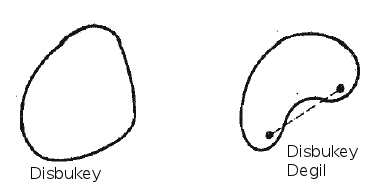
\includegraphics[height=3cm]{4_1.png}

Ve eger bu ``arada olmak'' denklemi, kumedeki her noktanin her diger
noktayla arasindaki, yani her $\alpha$ icin hesaplanacak noktalar icin de
dogru ise, o zaman hep ayni kumedeyi, ``disari cikmiyoruz'' demektir ve bu
disbukeyligin tanimidir. Gorsel olarak ta kabaca bunu gormek mumkundur,
disbukey bir cisimde bir noktadan digerine duz cizgide giderken hep cisim
icinde kaliriz.

Teori 

$K.G$ bir vektor uzayinda disbukey olan iki kume olsun. O zaman 

1. $\alpha K = \{x: x = \alpha k, k \in K\}$ her $\alpha$ icin disbukeydir. 

2. $K+G$ disbukeydir. 

Ispatlamadan bunun daha genel bir hali olan baska bir teoriye bakalim, onu
ispatlarsak usttekini de ispatlamis olacagiz. 

Teori 

$\mathscr{C}$, icindeki tum kumeleri disbukey olan rasgele bir buket
olsun. O zaman $\cap_{K \in \mathscr{C}}K$ ayni sekilde disbukeydir. 

Ispat

Diyelim ki $C = \cap_{K \in \mathscr{C}}K$. Eger $C$ bos ise, teori hemen
ispatlamistir. Diger sartlar icin, farzedelim ki $x_1,x_2 \in C$. O zaman
$x_1,x_2 \in K$ demektir, cunku $C$ bir kesisim, yani tum $K \in \mathscr{C}$
icindeki ayni olan ogelerden mutesekkil. Her $K$'nin kendi basina disbukey
oldugunu bildigimize gore, o zaman $C$ de disbukey demektir. 

\[ \square \]

Norm Edilmis Lineer Uzaylar

Soyut Analiz ve uygulamalarda ilgilenilen vektor uzaylarinin 7 onsarttan
daha fazlasina ihtiyaci vardir. 7 onsart vektor uzaylarinin sadece cebirsel
ozelliklerini tanimlar: toplam, skalar carpim, ve bunlarin degisik
kombinasyonlari. Eksik olanlar topolojik olan ozelliklerdir, yani aciklik
(openness), kapalilik (closure), yaklasiksallik (convergence), ve butunluk
(completeness). Eger uzayin icinde uzaklik olcumu tanimlanir ise, bu
kavramlar kullanilabilir. 

Tanim

Norm edilmis bir lineer uzay $X$ adindaki bir vektor uzayidir, ki $X$
icindeki her $x$ ogesini bir reel sayi $||x||$'e esleyen bir fonksiyon
vardir, ve $||x||$'e $x$'in norm'u adi verilir. Norm su onsartlari yerine
getirmelidir. 

1. $||x|| > 0$, her $x \in X$ icin, ve $||x|| = 0$, sadece ve sadece $x =
\theta$ ise. 

2. $||x+y|| \le ||x|| + ||y||$ her $x,y \in X$ icin (ucgensel esitsizlik) 

3. $||\alpha x|| = |\alpha| \ ||x||$, her skalar $\alpha$ ve her $x \in X$ icin. 

Norm kavrami uzaklik kavraminin soyutlastirilmis bir halinden ibaret
aslinda. Reel analizdeki ucgensel esitsizligin karsiligi burada da
goruluyor mesela. Neyse, devam edelim, ustteki ucgensel esitsizlik
kuralinin bir uzantisi / sonucu (lemma) su:

Teori 

Norm edilmis bir lineer uzayda $||x|| - ||y|| \le ||x-y|| \ \ \ \label{1}$ 

Ispat

\[ ||x|| - ||y|| = ||x - y + y|| - ||y||\]

Ustte adece $||x||$ icine $-y+y$ ekliyoruz, yani aslinda hicbir sey
degistirmedik. Simdi esitligin sagindaki ilk terimi alip ona ucgensel
esitligi uygularsak (norm icindeki $+$ isareti solu ve sagindaki gruplari
ayri terimler olarak kabul etmemiz gerekir)

\[ ||x - y + y|| - ||y|| \le
||x - y || + ||y|| - ||y|| 
\]

elde ederiz. Biraz daha basitlestirince

\[ ||x|| - ||y||  \le ||x - y ||  \]

$\square$

Uygun bir norm bulunabilirse, daha once gosterdigimiz vektor uzayi
orneklerinin cogunlugu norm edilebilen uzaya donusturulebilir.

Ornek 1

$C[a,b]$ adi verilen norm edilmis uzay, $[a,b]$ reel araligi, arti norm

\[ ||x|| = \max_{a \le t \le b} |x(t)| \]

tanimindan olusur. Hatirlarsak bu uzay daha once bir vektor uzayi olarak
gosterilmisti. Norm $[a,b]$ araligina bakiyor, her $x(t)$ icin mutlak degeri
(absolute value) en yuksek olan degeri alip onu norm degeri ilan
ediyor. Fonksiyon bir parabol ise, parabolun tepe noktasi o fonksiyon icin
norm kabul edilecek. 

Simdi teklif edilen norm'un 3 gerekli onsarti yerine getirip getirmedigine
bakalim. Bariz ki $||x|| \ge 0$ cunku norm kesin deger kullandik ve kesin
degerler hep sifirdan buyuk, ayrica $||x||$ sifir olmasi icin $x(t)$'nin
her yerde sifir olmasi lazim, fonksiyon tek bir noktada sifirdan azicik
daha buyuk olsaydi, $max$ hemen onu norm kabul ederdi. Ucgensel esitsizlik
alttaki iliskinin bir uzantisi zaten

\[ 
\max |x(t) + y(t)| \le 
\max [|x(t)| + |y(t)|] \le
\max |x(t)| + max |y(t)|
\]

Ustteki esitsizlikler maksimum fonksiyonun ozellikleri, ve bu ozellikler
onun ucgensel esitsizligi de yerine getirmesini sagliyor. 

En son olarak 3. onsart alttaki iliskinin dogal sonucu olarak yerine
getirilmis oluyor 

\[ \max |\alpha x(t)|  = \max |\alpha||x(t)| = |\alpha| \max |x(t)|  \]

Ornek

$[a,b]$ araliginda tanimli tum surekli fonksiyonlarin uzayi alttaki norm
uzerinden bir norm edilmis uzaydir

\[ ||x|| = \int _{ a}^{b} |x(t)|dt \]

Dikkat, bu norm edilmis uzay $C[a,b]$'den farklidir. 

Ornek 

Oklitsel n-uzayi ki $E^n$ olarak temsil edilir, ve norm'u $x = \{ \xi_1,
\xi_2, .., \xi_n\}$ 
icin $||x|| = (\sum _{ i=1}^{n} |\xi_i|^2)^{1/2}$, bir norm edilmis uzaydir. 

Yaklasiksallik (Convergence)

Cogu zaman, istenen bir ozellige sahip olan bir vektorun varligini ispat
ederken belli bir limite yaklasan bir vektor dizisi yaratmak yaygin bir
tekniktir. Cogu zaman bu limitin istenen ozellige sahip oldugu
gosterilebilir. Bu sebeple yaklasiksallik kavrami Analizde cok onemli rol
oynayan bir kavramdir. 

Tanim 

Norm edilmis bir lineer uzayda sonsuz sayida vektor iceren bir dizi
$\{x_n\}$'in $x$'e {\em yaklastigi} soylenir eger $\{||x_n-x||\}$ reel
sayilar dizisi sifira yaklasiyorsa. Bu durumda $x_n \to x$ diyebiliriz.

Eger $x_n \to x$, $||x_n|| \to ||x||$ olmali, cunku (1)'e gore 

\[ ||x_n||  - ||x|| \le ||x_n-x|| \]

ya da, terimlerin yeri degistirilmis halde

\[ ||x||  - ||x_n|| \le ||x-x_n|| \]

O zaman 

\[ \bigg| ||x||  - ||x_n|| \bigg|  \le ||x-x_n|| \to 0\]

olmalidir. 

Teori 

Eger bir dizi yaklasiyorsa, limiti ozgundur (unique)

Ispat

Diyelim ki $x_n \to x$ ve $x_n \to y$, yani $x_n$ apayri iki limite
yaklasiyor (gibi) bir sey ortaya attik. Peki o zaman $||x-y||$ ne olur?
Gorecegiz ki bu norm sifira gidecek ve bu sebeple $x,y$'nin birbirinden
farkli olamayacagini anlamis olacagiz. 

\[ ||x-y|| =  ||x-x_n + x_n-y|| \]

Ustte yine ayni numarayi kullandik, $-x_n+x_n$ ekleyerek esitlikte hicbir
sey degistirmiyoruz, ama daha fazla terim elde ederek simdi ucgensel
esitsizligi kullanabilecegiz. $+$ isaretinin solundaki ve sagindaki
bloklari ayri terimler gibi kabul edersek, 

\[ ||x-x_n + x_n-y|| \le ||x-x_n || + ||x_n-y|| \]

ve

\[ ||x-x_n || \to 0 \]

\[ ||x_n-y|| \to 0\]

olduguna gore 

\[ ||x-y|| \to 0 \]

$\square$





\end{document}
